
\pagebreak

\section{Views}

\subsection{Logical view}


\begin{figure}[H]
%\vspace{-30pt}
\begin{center}
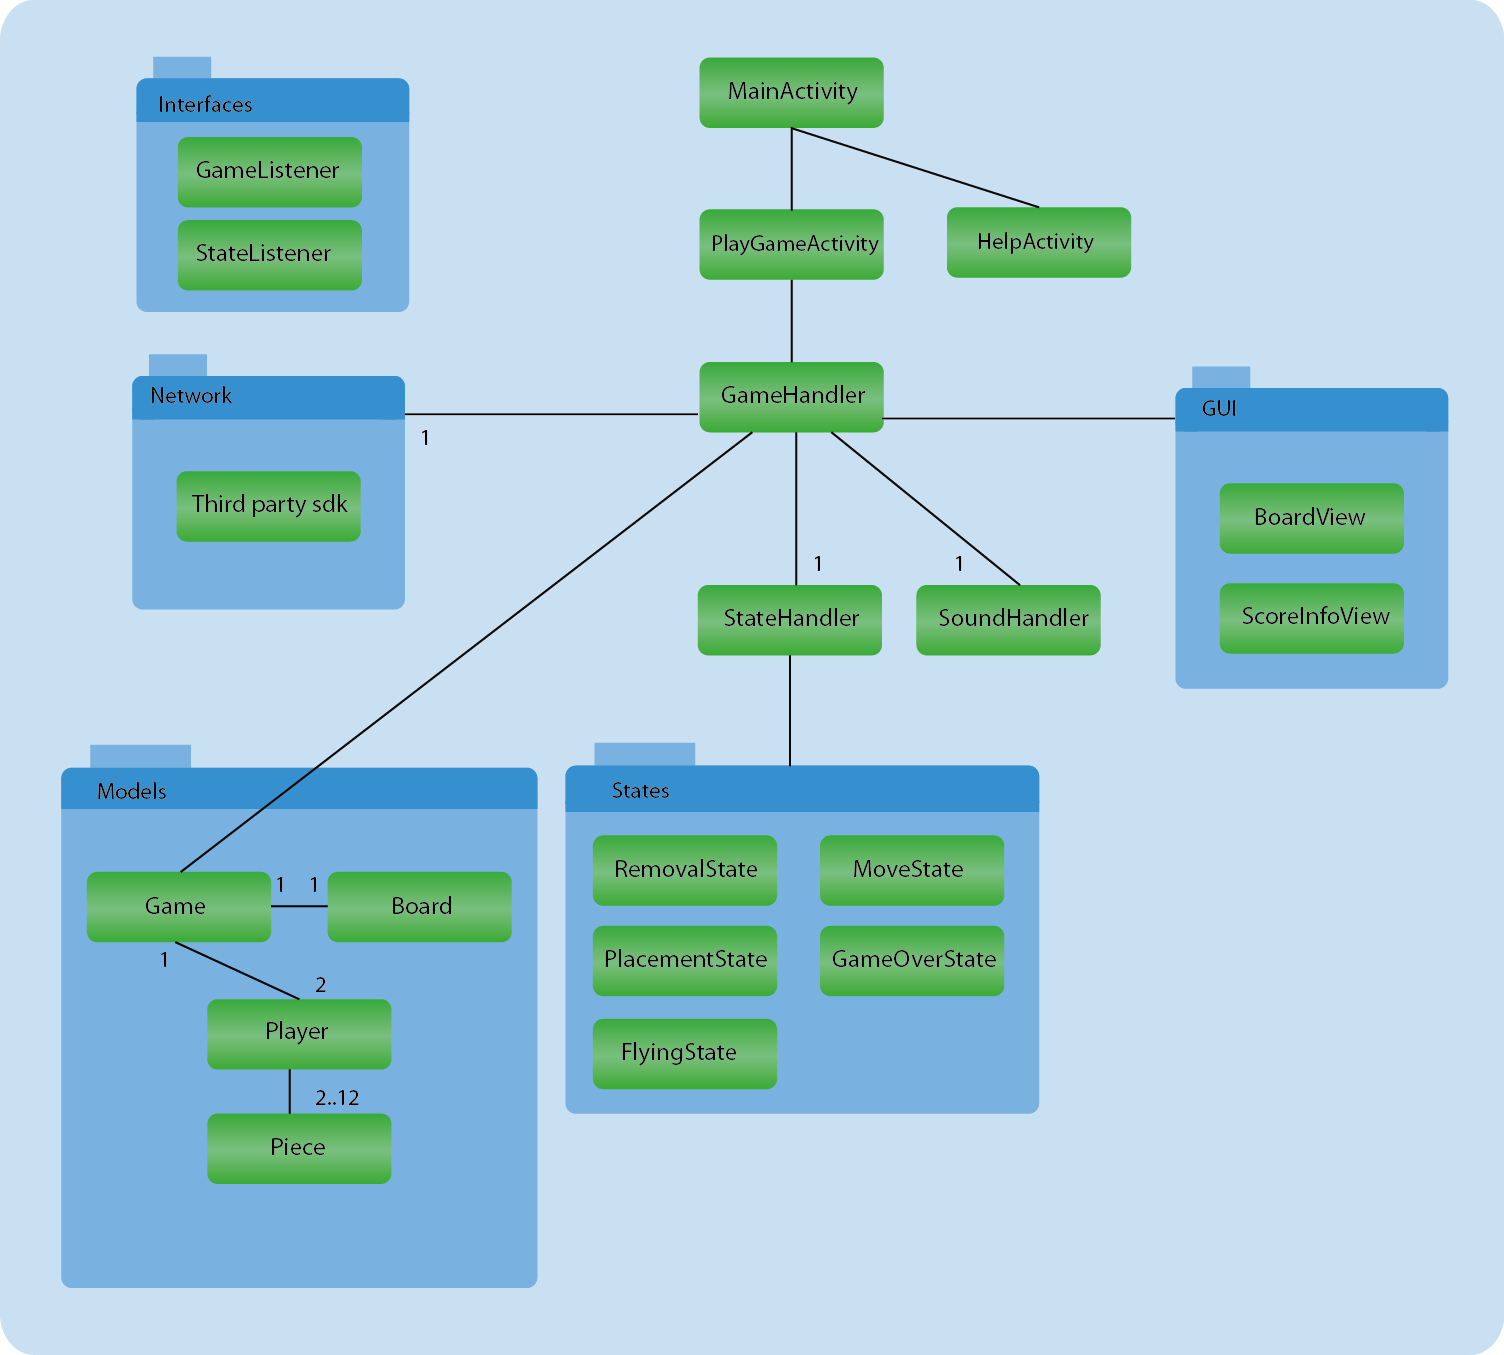
\includegraphics[width=\textwidth]{./Images/LogicalView.png}
\end{center}
\caption{Logical view}
\end{figure}

The diagram follows the 4+1 logic view notation suggested by the Kructhen article \cite{krutchen}. The class diagram shows the structure of a system by showing the system's classes  and the relationships among them. Aggregation and inheritance is also displayed.

\subsection{Development view}

\begin{figure}[H]
\begin{center}
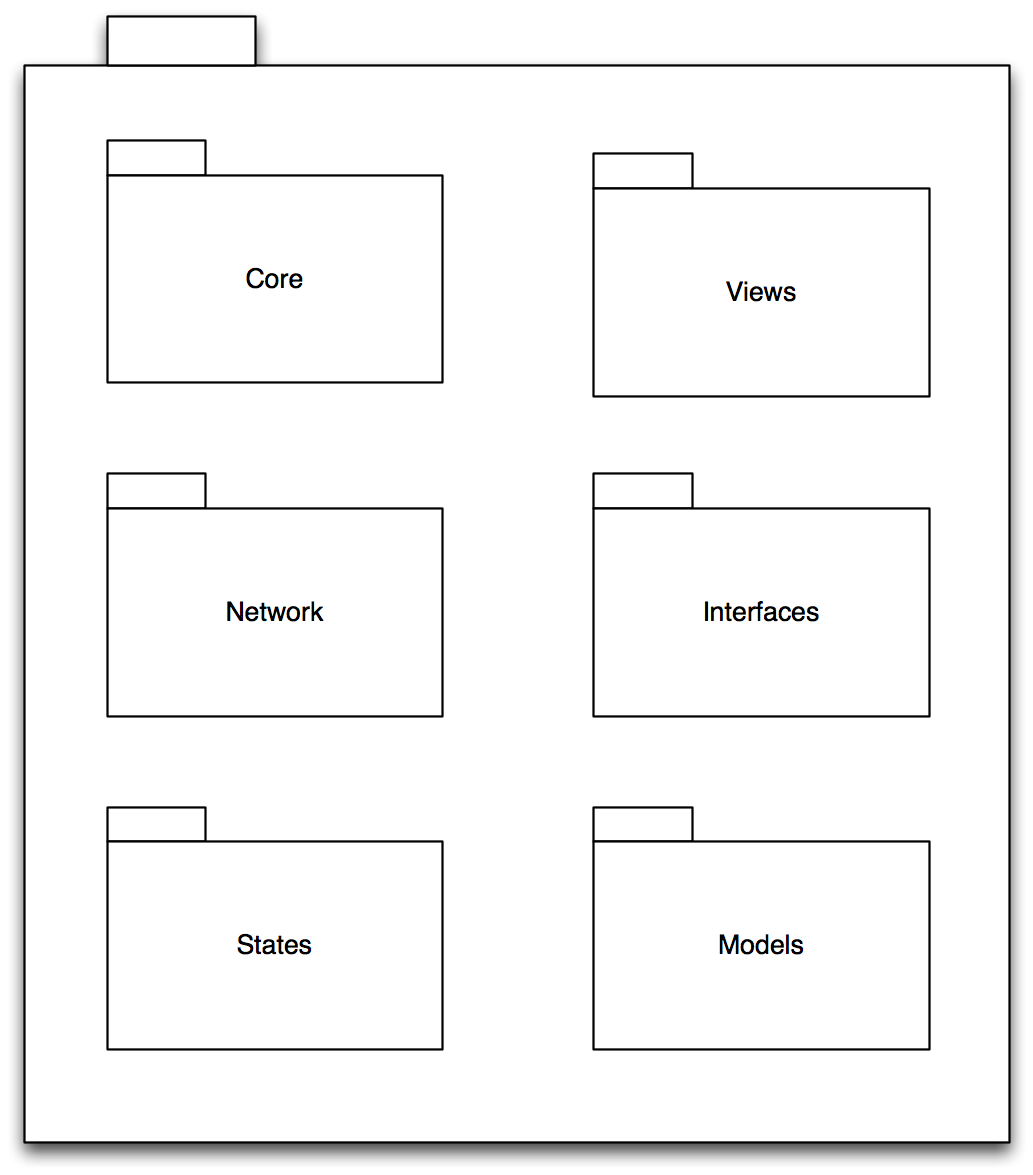
\includegraphics[width=220pt]{./Images/DevelopmentView.png}
\end{center}
\caption{Development view}
\end{figure}

The game is divided into several layers. The android framework, a 2D framework, the game logic, and graphics. The diagram show the different parts of the system.

\pagebreak

\subsection{Process view}

\begin{figure}[H]
%\vspace{-30pt}
\begin{center}
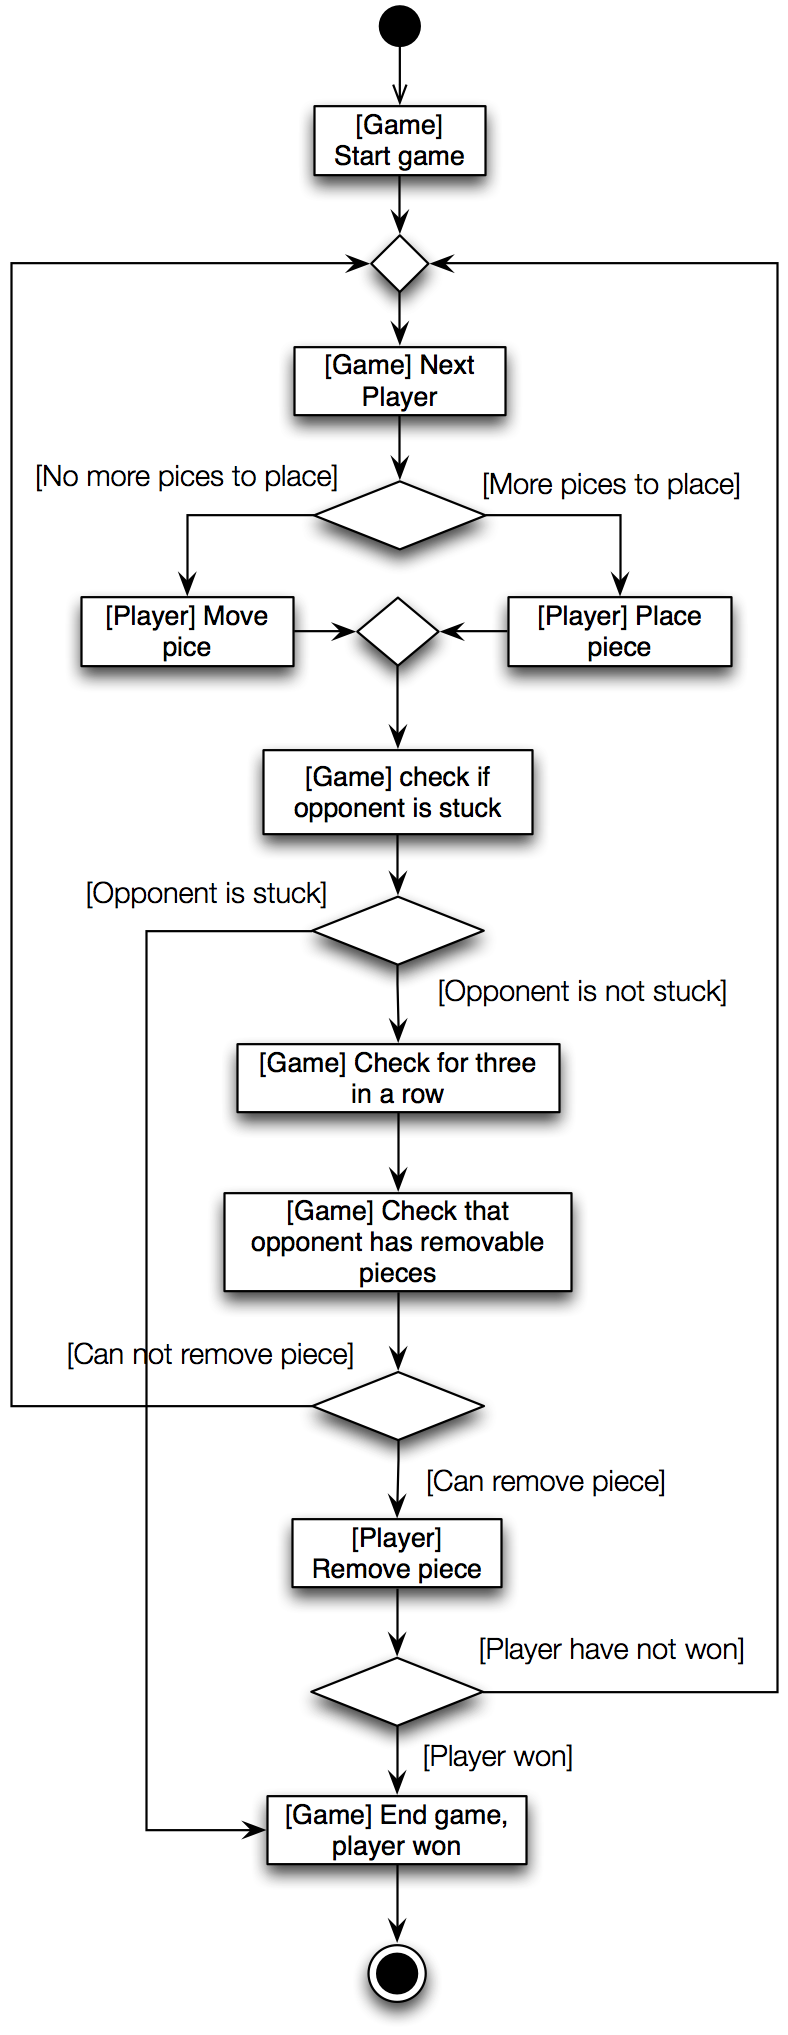
\includegraphics[width=200pt]{./Images/ProcessView}
\end{center}
\caption{Process view}
\end{figure}

The game is a turn based game with two players. In the activity diagram the progress of a game is described. When a game is started one of the players starts placing one of its pieces. The game checks if the player get three in a row. In that case the player can remove one of the opponents pieces. If the opponents have less then three pieces left, the other player have won. The diagram shows how a game round will pan out. 

\subsection{Physical view}

\begin{figure}[H]
%\vspace{-30pt}
\begin{center}
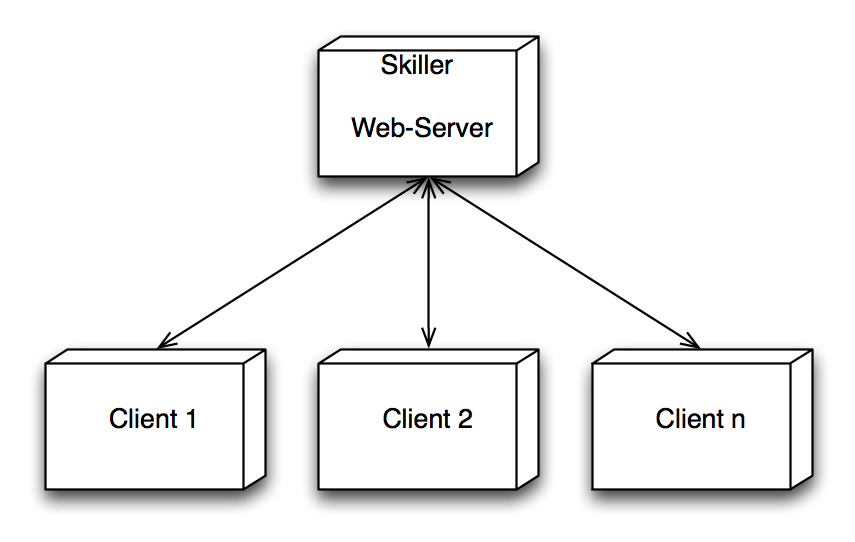
\includegraphics[width=200pt]{./Images/physicalLayer1}
\end{center}
\caption{Physical view}
\end{figure}

The deployment diagram illustrates communication between the third part web-server and the clients. Skiller is a mobile social gaming platform. Skiller’s platform enables users to play (multiplayer) and fully interact with each other using a large variety of social features (messaging, buddy list, personal profile, avatars and more). By using skiller we avoid developing our own web-server. Skiller have a small but powerfoul api that make our turn based communication easy. It also make creating and joining games easy. When a client creates a game, a game will be created on the client and server side. The local game, will be independent from the servers, which means that skiller can be replaced with another server library. If a player wants to joine a game he will get a list of created games in the skiller 'lobby'. When a player select a game bouth players will be connected to the server. The web-server sends a message to both players that the game have startet. After that, messages will be sent between the clients when the other have done an act.




